\documentclass[tikz,border=3pt]{standalone}
\usepackage[T1]{fontenc}
\usepackage{newtxtext,newtxmath}
\usetikzlibrary{arrows.meta,calc,patterns}
\definecolor{ink}{HTML}{23343F}
\definecolor{blue}{HTML}{2276A0}
\definecolor{teal}{HTML}{087F78}
\definecolor{orange}{HTML}{C46B2C}
\definecolor{muted}{HTML}{4C5D67}
\definecolor{rule}{HTML}{CFDADF}
\begin{document}
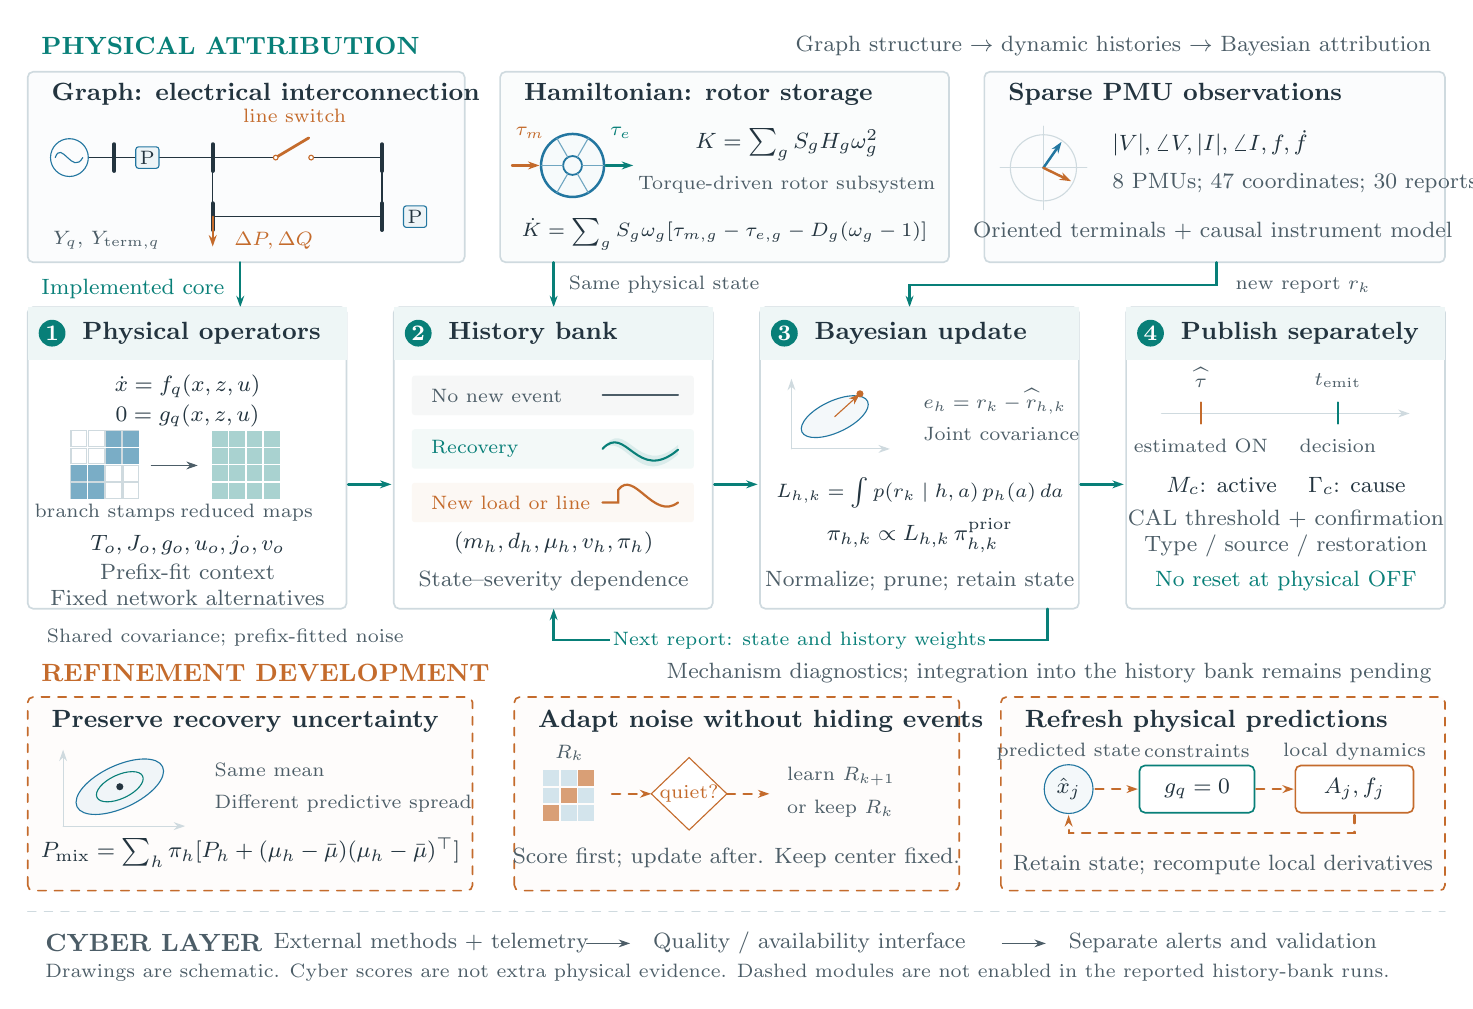
\begin{tikzpicture}[font=\fontsize{8.3}{10}\selectfont,text=ink,line cap=round,
 >={Stealth[length=1.45mm,width=1mm]},
 head/.style={font=\bfseries\fontsize{9}{11}\selectfont,anchor=west},
 note/.style={font=\fontsize{7.8}{9.4}\selectfont,text=muted},
 small/.style={font=\fontsize{7.2}{8.5}\selectfont,text=muted},
 card/.style={draw=rule,rounded corners=2pt,fill=white,line width=.6pt},
 flow/.style={->,draw=teal,line width=.85pt},
 future/.style={->,draw=orange,dashed,line width=.75pt},
 bus/.style={draw=ink,line width=1.4pt}]
\path[use as bounding box] (0,0) rectangle (18,12.1);
\node[head,text=teal] at (.05,11.87) {PHYSICAL ATTRIBUTION};
\node[note,anchor=east] at (17.95,11.87) {Graph structure $\rightarrow$ dynamic histories $\rightarrow$ Bayesian attribution};

% Context band: real electrical primitives, a common event clock, PMU phasors.
\path[card,fill=blue!2] (0,9.12) rectangle (5.55,11.54);
\path[card,fill=teal!2] (6.0,9.12) rectangle (11.7,11.54);
\path[card,fill=blue!2] (12.15,9.12) rectangle (18,11.54);
\node[head] at (.18,11.25) {Graph: electrical interconnection};
\foreach \x/\y in {1.1/10.45,2.35/10.45,4.5/10.45,2.35/9.7,4.5/9.7}{
 \draw[bus] (\x,{\y-.17})--(\x,{\y+.17});}
\draw[ink] (.77,10.45)--(1.1,10.45)--(2.35,10.45)--(3.15,10.45)
 (3.6,10.45)--(4.5,10.45)--(4.5,9.7)--(2.35,9.7)--(2.35,10.45);
\draw[blue] (.53,10.45) circle (.24);
\draw[blue] (.35,10.45) .. controls (.43,10.68) and (.57,10.22) .. (.7,10.45);
\draw[orange,line width=1pt] (3.15,10.45)--(3.57,10.70);
\draw[orange,fill=white] (3.15,10.45) circle (.03) (3.6,10.45) circle (.03);
\draw[orange,->,line width=.8pt] (2.35,9.7)--(2.35,9.32);
\node[small,anchor=west,text=orange] at (2.5,9.40) {$\Delta P,\Delta Q$};
\node[small,text=orange] at (3.39,10.98) {line switch};
\foreach \x/\y in {1.1/10.45,4.5/9.7}{
 \node[draw=blue,fill=blue!8,rounded corners=1pt,inner sep=1.5pt,font=\fontsize{6.8}{8}\selectfont] at ({\x+.42},\y) {P};}
\node[small,anchor=west] at (.2,9.40) {$Y_q$, $Y_{{\rm term},q}$};
\node[head] at (6.18,11.25) {Hamiltonian: rotor storage};
\draw[blue,line width=.9pt,fill=blue!4] (6.92,10.35) circle (.40);
\draw[blue,line width=.65pt] (6.92,10.35) circle (.12);
\foreach \a in {0,60,...,300}{\draw[blue!65] (6.92,10.35) ++(\a:.12)--++(\a:.28);}
\draw[orange,->,line width=.8pt] (6.15,10.35)--(6.50,10.35);
\draw[teal,->,line width=.8pt] (7.34,10.35)--(7.69,10.35);
\node[small,text=orange] at (6.38,10.76) {$\tau_m$};
\node[small,text=teal] at (7.53,10.76) {$\tau_e$};
\node at (9.64,10.61) {$K=\sum_g S_gH_g\omega_g^2$};
\node[small] at (9.64,10.11) {Torque-driven rotor subsystem};
\node[font=\fontsize{7.2}{8.5}\selectfont] at (8.85,9.48)
 {$\dot K=\sum_g S_g\omega_g[\tau_{m,g}-\tau_{e,g}-D_g(\omega_g-1)]$};
\node[head] at (12.33,11.25) {Sparse PMU observations};
\draw[rule] (12.90,10.32) circle (.42);
\draw[rule] (12.35,10.32)--(13.45,10.32) (12.9,9.79)--(12.9,10.85);
\draw[blue,->,line width=.9pt] (12.9,10.32)--(13.13,10.65);
\draw[orange,->,line width=.9pt] (12.9,10.32)--(13.25,10.15);
\node[anchor=west] at (13.65,10.63) {$|V|,\angle V,|I|,\angle I,f,\dot f$};
\node[note,anchor=west] at (13.65,10.13) {8 PMUs; 47 coordinates; 30 reports/s};
\node[note] at (15.05,9.52) {Oriented terminals + causal instrument model};

% Separate measurement route goes directly to the scoring card.
\draw[flow] (2.70,9.12)--(2.70,8.55);
\draw[flow] (6.68,9.12)--(6.68,8.55);
\node[small,anchor=west,fill=white,inner sep=1pt] at (6.83,8.83) {Same physical state};
\draw[flow] (15.1,9.12)--(15.1,8.83)--(11.2,8.83)--(11.2,8.55);
\node[small,anchor=west,fill=white,inner sep=1pt] at (15.3,8.83) {new report $r_k$};
\node[note,anchor=west,text=teal] at (.05,8.78) {Implemented core};

% Four processing cards: equations paired with a distinct visual mechanism.
\foreach \a/\b/\num in {0/4.05/1,4.65/8.7/2,9.3/13.35/3,13.95/18/4}{
 \path[card] (\a,4.72) rectangle (\b,8.55);
 \fill[teal!7] (\a,7.88) rectangle (\b,8.55);
 \node[circle,fill=teal,text=white,inner sep=0pt,minimum size=.34cm,font=\bfseries\fontsize{8}{9}\selectfont] at ({\a+.31},8.22) {\num};
}
\node[head] at (.57,8.22) {Physical operators};
\node[head] at (5.22,8.22) {History bank};
\node[head] at (9.87,8.22) {Bayesian update};
\node[head] at (14.52,8.22) {Publish separately};
\node at (2.03,7.55) {$\dot x=f_q(x,z,u)$};
\node at (2.03,7.17) {$0=g_q(x,z,u)$};
% Sparse stamp -> reduced operator glyph (not an IEEE-39 graph).
\foreach \i in {0,1,2,3}{\foreach \j in {0,1,2,3}{
 \draw[rule,fill=white] ({.55+.22*\i},{6.12+.22*\j}) rectangle ++(.20,.20);}}
\foreach \i/\j in {0/0,1/1,2/2,3/3,1/0,0/1,3/2,2/3}{
 \fill[blue!60] ({.55+.22*\i},{6.12+.22*\j}) rectangle ++(.20,.20);}
\draw[->,muted] (1.57,6.54)--(2.16,6.54);
\foreach \i in {0,1,2,3}{\foreach \j in {0,1,2,3}{
 \fill[teal!35] ({2.34+.22*\i},{6.12+.22*\j}) rectangle ++(.20,.20);}}
\node[small] at (.98,5.94) {branch stamps};\node[small] at (2.78,5.94) {reduced maps};
\node at (2.03,5.53) {$T_o,J_o,g_o,u_o,j_o,v_o$};
\node[note,align=center] at (2.03,5.02) {Prefix-fit context\\Fixed network alternatives};

% Three histories and their schematic predictive spread.
\foreach \y/\txt/\cc in {7.43/{No new event}/muted,6.75/{Recovery}/teal,6.07/{New load or line}/orange}{
 \fill[\cc!5,rounded corners=1pt] (4.88,{\y-.25}) rectangle (8.46,{\y+.25});
 \node[small,text=\cc,anchor=west] at (5.0,\y) {\txt};}
\draw[muted,line width=.65pt] (7.3,7.43)--(8.26,7.43);
\fill[teal!15] (7.3,6.75) .. controls (7.6,7.20) and (7.74,6.35) .. (8.26,6.80)
 --(8.26,6.68) .. controls (7.74,6.22) and (7.6,6.98) .. (7.3,6.75);
\draw[teal,line width=.75pt] (7.3,6.75) .. controls (7.6,7.08) and (7.74,6.30) .. (8.26,6.74);
\draw[orange,line width=.8pt] (7.3,6.07)--(7.5,6.07)--(7.5,6.23) .. controls (7.7,6.50) and (7.95,5.83) .. (8.26,6.07);
\node at (6.68,5.55) {$(m_h,d_h,\mu_h,v_h,\pi_h)$};
\node[note] at (6.68,5.07) {State--severity dependence};

% Innovation geometry icon; the scoring equation remains central.
\draw[rule,->] (9.7,6.75)--(10.95,6.75);\draw[rule,->] (9.7,6.75)--(9.7,7.64);
\draw[blue,rotate around={25:(10.25,7.16)},fill=blue!5] (10.25,7.16) ellipse (.46 and .20);
\fill[orange] (10.57,7.45) circle (.045);
\draw[orange,->] (10.25,7.16)--(10.57,7.45);
\node[small,anchor=west] at (11.25,7.35) {$e_h=r_k-\widehat r_{h,k}$};
\node[small,anchor=west] at (11.25,6.94) {Joint covariance};
\node[font=\fontsize{7.4}{8.5}\selectfont] at (11.33,6.19) {$L_{h,k}=\int p(r_k\mid h,a)\,p_h(a)\,da$};
\node at (11.33,5.65) {$\pi_{h,k}\propto L_{h,k}\,\pi_{h,k}^{\rm prior}$};
\node[note] at (11.33,5.07) {Normalize; prune; retain state};

% Decision timeline: emission is explicitly distinct from inferred onset.
\draw[rule,->] (14.4,7.20)--(17.55,7.20);
\draw[orange,line width=.7pt] (14.90,7.07)--(14.90,7.34);
\draw[teal,line width=.7pt] (16.64,7.07)--(16.64,7.34);
\node[small,above] at (14.90,7.4) {$\widehat\tau$};\node[small,above] at (16.64,7.4) {$t_{\rm emit}$};
\node[small,below] at (14.90,7.0) {estimated ON};\node[small,below] at (16.64,7.0) {decision};
\node at (15.98,6.28) {$M_c$: active \quad $\Gamma_c$: cause};
\node[note,align=center] at (15.98,5.68) {CAL threshold + confirmation\\Type / source / restoration};
\node[note,text=teal] at (15.98,5.07) {No reset at physical OFF};
\foreach \x in {4.05,8.7,13.35}{\draw[flow] ({\x+.02},6.3)--({\x+.57},6.3);}
\draw[flow] (12.95,4.72)--(12.95,4.32)--(6.68,4.32)--(6.68,4.72);
\node[small,text=teal,fill=white,inner sep=1pt] at (9.8,4.32) {Next report: state and history weights};
\node[small,anchor=west] at (.12,4.35) {Shared covariance; prefix-fitted noise};

% Development lane: mechanism drawings rather than another wall of prose.
\node[head,text=orange] at (.05,3.91) {REFINEMENT DEVELOPMENT};
\node[note,anchor=east] at (17.95,3.91) {Mechanism diagnostics; integration into the history bank remains pending};
\foreach \a/\b in {0/5.65,6.18/11.83,12.36/18}{
 \path[card,draw=orange,dashed,fill=orange!2] (\a,1.14) rectangle (\b,3.60);}
\node[head] at (.18,3.29) {Preserve recovery uncertainty};
\draw[rule,->] (.45,1.96)--(2.0,1.96);\draw[rule,->] (.45,1.96)--(.45,2.93);
\draw[blue,rotate around={25:(1.17,2.46)},fill=blue!7] (1.17,2.46) ellipse (.60 and .27);
\draw[teal,rotate around={25:(1.17,2.46)}] (1.17,2.46) ellipse (.32 and .15);
\fill[ink] (1.17,2.46) circle (.045);
\node[small,anchor=west] at (2.25,2.67) {Same mean};
\node[small,anchor=west] at (2.25,2.25) {Different predictive spread};
\node at (2.83,1.62) {$P_{\rm mix}=\sum_h\pi_h[P_h+(\mu_h-\bar\mu)(\mu_h-\bar\mu)^\top]$};
\node[head] at (6.36,3.29) {Adapt noise without hiding events};
% A covariance factor and a gate are separate visual objects.
\foreach \i in {0,1,2}{\foreach \j in {0,1,2}{\fill[blue!20] ({6.55+.22*\i},{2.03+.22*\j}) rectangle ++(.20,.20);}}
\foreach \i in {0,1,2}{\fill[orange!65] ({6.55+.22*\i},{2.03+.22*\i}) rectangle ++(.20,.20);}
\node[small] at (6.88,2.89) {$R_k$};
\draw[future] (7.42,2.37)--(7.92,2.37);
\draw[orange,fill=white] (8.40,2.83)--(8.88,2.37)--(8.40,1.91)--(7.92,2.37)--cycle;
\node[small,text=orange,align=center] at (8.40,2.37) {quiet?};
\draw[future] (8.88,2.37)--(9.42,2.37);
\node[small,anchor=west] at (9.52,2.59) {learn $R_{k+1}$};
\node[small,anchor=west] at (9.52,2.18) {or keep $R_k$};
\node[note] at (9.0,1.55) {Score first; update after. Keep center fixed.};
\node[head] at (12.54,3.29) {Refresh physical predictions};
\node[small] at (13.22,2.91) {predicted state};
\node[small] at (14.85,2.91) {constraints};
\node[small] at (16.85,2.91) {local dynamics};
\draw[blue,fill=blue!5] (13.22,2.43) circle (.31);
\node at (13.22,2.43) {$\hat x_j$};
\path[card,draw=teal] (14.12,2.13) rectangle (15.58,2.73);
\node at (14.85,2.43) {$g_q=0$};
\path[card,draw=orange] (16.10,2.13) rectangle (17.60,2.73);
\node at (16.85,2.43) {$A_j,f_j$};
\draw[future] (13.56,2.43)--(14.10,2.43);
\draw[future] (15.60,2.43)--(16.08,2.43);
\draw[future] (16.85,2.10)--(16.85,1.87)--(13.22,1.87)--(13.22,2.10);
\node[note] at (15.18,1.47) {Retain state; recompute local derivatives};

% Deliberately detached external service: no attack-to-event score arrow.
\draw[rule,dashed] (0,.88)--(18,.88);
\node[head,text=muted] at (.10,.47) {CYBER LAYER};
\node[note,anchor=west] at (3.0,.47) {External methods + telemetry};
\draw[->,muted] (7.1,.47)--(7.65,.47);
\node[note,anchor=west] at (7.82,.47) {Quality / availability interface};
\draw[->,muted] (12.38,.47)--(12.93,.47);
\node[note,anchor=west] at (13.10,.47) {Separate alerts and validation};
\node[small,anchor=west] at (.10,.10) {Drawings are schematic. Cyber scores are not extra physical evidence. Dashed modules are not enabled in the reported history-bank runs.};
\end{tikzpicture}
\end{document}
